% fig_coord_ladder.tex
% TR-35: Time ladder — five protection functions on a common timeline
%
% X-axis: time [ms], 0 to ~430
% Five swim-lanes at hardcoded y-positions (no digit-containing macros)
%
% Functions and trip times:
%   87L       : 20 ms  (all faults, k>=0.06)            green
%   Z1 Quad   : 20 ms  (metallic, alpha<=0.80, k>=0.10) blue
%   67N/67Q   : 30 ms  (SLG/LL, k>=0.04)               orange
%   Z2/POTT   : 32 ms  (3PH, alpha>0.80, k>=0.10)      teal
%   TDCS      : 400 ms (backup)                         red/dashed
%
% Scale: 1 cm = 40 ms  →  0ms=0.00, 20ms=0.50, 30ms=0.75, 32ms=0.80,
%        100ms=2.50, 300ms=7.50, 400ms=10.00, end=11.00

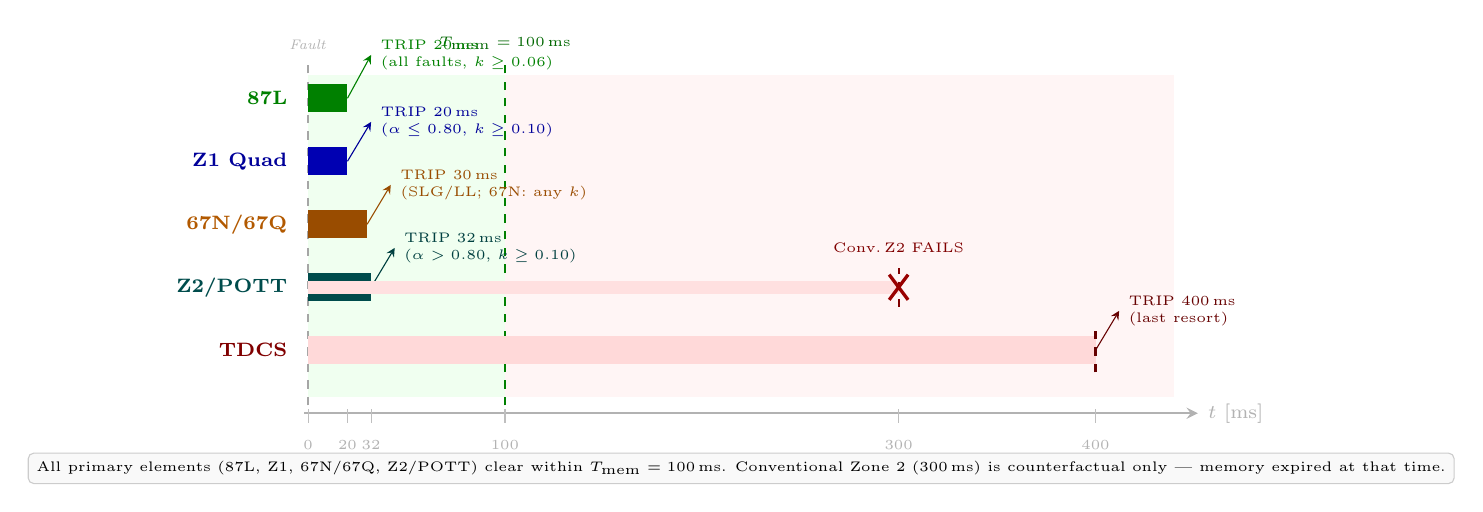
\begin{tikzpicture}[every node/.style={font=\scriptsize}]

%% ── Hardcoded x-positions (cm, scale 1cm=40ms) ───────────────────────────────
% xFault=0, xTrip20=0.50, xTrip30=0.75, xTrip32=0.80
% xMem=2.50, xConvZ2=7.50, xTDCS=10.00, xEnd=11.00

%% ── Hardcoded lane y-positions (letters only) ────────────────────────────────
% yDiffL=4.0, yZone=3.2, yDir=2.4, yPott=1.6, yTDCS=0.8, yAx=0.0

%% ── Memory window ─────────────────────────────────────────────────────────────
\fill[green!6]  (0, 0.20) rectangle (2.50, 4.30);
\fill[red!4]    (2.50, 0.20) rectangle (11.00, 4.30);
\draw[green!50!black, dashed, thick] (2.50, 0.10) -- (2.50, 4.50);
\node[green!40!black, font=\tiny, above] at (2.50, 4.50)
  {$T_\mathrm{mem}=100$\,ms};

%% ── Fault inception ──────────────────────────────────────────────────────────
\draw[gray!70, thick, dashed] (0, 0.10) -- (0, 4.50);
\node[gray!60, above, font=\tiny] at (0, 4.50) {\textit{Fault}};

%% ── Time axis ─────────────────────────────────────────────────────────────────
\draw[->, >=stealth, gray!60, thick]
  (-0.05, 0.0) -- (11.30, 0.0) node[right, gray!60] {$t$ [ms]};

\foreach \xpos/\lab in {0.00/0, 0.50/20, 0.80/32, 2.50/100, 7.50/300, 10.00/400}{
  \draw[gray!50, thin] (\xpos, -0.12) -- (\xpos, 0.05);
  \node[gray!60, below=3pt, font=\tiny] at (\xpos, -0.12) {\lab};
}

%% ── Lane labels ──────────────────────────────────────────────────────────────
\node[green!50!black, font=\scriptsize\bfseries, left=4pt] at (0, 4.0) {87L};
\node[blue!60!black,  font=\scriptsize\bfseries, left=4pt] at (0, 3.2) {Z1 Quad};
\node[orange!70!black,font=\scriptsize\bfseries, left=4pt] at (0, 2.4) {67N/67Q};
\node[teal!60!black,  font=\scriptsize\bfseries, left=4pt] at (0, 1.6) {Z2/POTT};
\node[red!50!black,   font=\scriptsize\bfseries, left=4pt] at (0, 0.8) {TDCS};

%% ── 87L bar (0 to 20 ms) ─────────────────────────────────────────────────────
\fill[green!50!black] (0, 3.82) rectangle (0.50, 4.18);
\draw[green!50!black, ->, >=stealth]
  (0.50, 4.0) -- (0.80, 4.55)
  node[right, green!50!black, font=\tiny, align=left]
  {TRIP 20\,ms\\(all faults, $k\geq0.06$)};

%% ── Z1 Quad bar ──────────────────────────────────────────────────────────────
\fill[blue!70!black] (0, 3.02) rectangle (0.50, 3.38);
\draw[blue!60!black, ->, >=stealth]
  (0.50, 3.2) -- (0.80, 3.7)
  node[right, blue!60!black, font=\tiny, align=left]
  {TRIP 20\,ms\\($\alpha\leq0.80$, $k\geq0.10$)};

%% ── 67N/67Q bar ──────────────────────────────────────────────────────────────
\fill[orange!60!black] (0, 2.22) rectangle (0.75, 2.58);
\draw[orange!60!black, ->, >=stealth]
  (0.75, 2.4) -- (1.05, 2.9)
  node[right, orange!60!black, font=\tiny, align=left]
  {TRIP 30\,ms\\(SLG/LL; 67N: any $k$)};

%% ── Z2/POTT bar ──────────────────────────────────────────────────────────────
\fill[teal!60!black] (0, 1.42) rectangle (0.80, 1.78);
\draw[teal!50!black, ->, >=stealth]
  (0.80, 1.6) -- (1.10, 2.1)
  node[right, teal!50!black, font=\tiny, align=left]
  {TRIP 32\,ms\\($\alpha>0.80$, $k\geq0.10$)};

%% ── Conv Z2 counterfactual (300 ms) ─────────────────────────────────────────
\fill[red!12] (0, 1.52) rectangle (7.50, 1.68);
\draw[red!50!black, thick, dashed]
  (7.50, 1.35) -- (7.50, 1.85);
\draw[red!60!black, very thick]
  (7.38, 1.44) -- (7.62, 1.76);
\draw[red!60!black, very thick]
  (7.38, 1.76) -- (7.62, 1.44);
\node[red!50!black, font=\tiny, above=2pt] at (7.50, 1.85)
  {Conv.\,Z2 FAILS};

%% ── TDCS backup bar ──────────────────────────────────────────────────────────
\fill[red!15] (0, 0.62) rectangle (10.00, 0.98);
\draw[red!40!black, thick, dashed]
  (10.00, 0.52) -- (10.00, 1.08);
\draw[red!40!black, ->, >=stealth]
  (10.00, 0.8) -- (10.30, 1.3)
  node[right, red!40!black, font=\tiny, align=left]
  {TRIP 400\,ms\\(last resort)};

%% ── Caption ──────────────────────────────────────────────────────────────────
\node[draw=gray!40, fill=gray!5, rounded corners=2pt,
      font=\tiny, inner sep=3pt, align=center]
  at (5.50, -0.70)
  {All primary elements (87L, Z1, 67N/67Q, Z2/POTT) clear within
   $T_\mathrm{mem}=100$\,ms.
   Conventional Zone~2 (300\,ms) is counterfactual only --- memory expired at that time.};

\end{tikzpicture}
